\documentclass[12pt, a4paper]{report}
\usepackage{fullpage}
\usepackage[final]{microtype}
\usepackage[hyperfootnotes=false]{hyperref}
\usepackage[pdftex]{graphicx}
\usepackage{multirow}
\usepackage{algorithm}
\usepackage{algorithmic}
\usepackage{parskip}
\usepackage{proof}
\usepackage{amsmath, amssymb, amsthm}
\usepackage{enumerate}
\usepackage{color}
\usepackage{setspace}
\usepackage[justification=centering]{caption}
\usepackage{subcaption}
\usepackage{footnotebackref}

% \onehalfspacing

\usepackage[hang]{footmisc}
\setlength\footnotemargin{10pt}

\newtheorem*{Brooks}{Brook's Theorem}
\newtheorem{claim}{Claim}

\begin{document}
\pagenumbering{roman}
\title{CS5234 Project\\ Airport Gate Scheduling}
\author{Choo XianJun, Davin \\ Lee Yik Jiun}
\date{}
\maketitle

% \listoffigures
% \listoftables
% \listofalgorithms

\setcounter{tocdepth}{1}
\tableofcontents 

\chapter{Introduction}
\pagenumbering{arabic}
\section{Background}
Scheduling is an interesting class of combinatorial optimization problems that have very practical use. One such scheduling problem is the \textbf{airport gate scheduling problem}.

In this problem, we have $n_1$ arriving flights and $n_2$ departure flights. Associated with each of these flights is a timing $x_i$, where $i \in \{1, ... , n_1 + n_2\}$, indicating the time of arrival or departure of the respective flight. Depending on the type of flight, different amount of buffer times are allocated, resulting in an interval of time which the plane needs to use a gate. Departing flight $i$ can be represented as the interval $[90 - x_i, x_i + 30)$ while arriving flight $j$ can be represented as the interval $[x_j, x_j + 45)$. The problem then requires us to minimise the number of gates needed to satisfy a given list of flights so that no intervals collide.

Beyond the above vanilla formulation of the airport gate scheduling problem, there are many variations and modifications to the problem. Life is hardly predictable and so are scheduled flight timings. Airports encounter several flight delays\footnote{Delays can be negative, which simply means the plane took off/landed earlier than expected!} daily. This presents an interesting variant of the problem which considers delays in the system.

\section{Organisation of report}
We first present some literature review and plausible approaches to the problem. After tackling the vanilla airport gate scheduling problem without delays, we delve into the more interesting variant which considers delays in the system. Along the way, we will provide sufficient mathematical rigour and point out interesting patterns and observations that we have.

\chapter{Vanilla Airport Gate Scheduling}
\section{Interval scheduling}
\subsection{Problem description}
Given a set of jobs which must take place between their respective interval periods of time, what is the maximum number of jobs that we can fulfill without any interval overlaps? In interval scheduling, we are restricted to only 1 processor. That is to say, everything must be scheduled on a single timeline. This is also known as the ``Interval Scheduling Maximizatin Problem (ISMP)''.

There are several other variants to this problem where the set of jobs is described as a union of different groups of jobs. The problem of ``Group Interval Scheduling Maximization Problem (GISMP)'' is then concerned about maximizing the number of groups such that at least one job in these groups is being executed.

In the context of interval scheduling airport gate scheduling can then be seen as interval scheduling with multiple processors, where we aim to minimize the number of processers needed. We illustrate this in Figure \ref{fig:FlightsAsIntervals}.

\begin{figure}[h!]
\centering
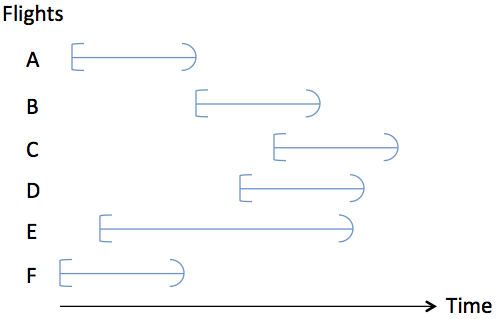
\includegraphics[width=0.4\textwidth]{../figures/vanilla.png}
\caption{Illustration of flights as time intervals}
\label{fig:FlightsAsIntervals}
\end{figure}

\subsection{Optimal solution}
It turns out the interval scheduling problem has a greedy optimal algorithm (Algorithm \ref{alg:Greedy Interval Scheduling}) of packing as many earliest ending jobs as possible.

\begin{algorithm}[h!]
\begin{algorithmic}[1]
\caption{\textsc{GreedyIntervalScheduling}(Jobs)}
\label{alg:Greedy Interval Scheduling}
\STATE $J \leftarrow \textsc{SortByEarliestFinishingTime(Jobs)}$
\STATE $Chosen \leftarrow \emptyset$
\WHILE{$J$ not empty}
	\STATE $x \leftarrow J.pop()$
	\STATE $Chosen \leftarrow Chosen \cup \{x\}$
	\FOR{$y \leftarrow J \setminus \{x\}$}
		\IF{$y$ overlaps with $x$}
			\STATE $J \leftarrow J \setminus \{y\}$
		\ENDIF
	\ENDFOR
\ENDWHILE
\RETURN $Chosen$
\end{algorithmic}
\end{algorithm}

\subsubsection{Proof of correctness}
It is obvious that if $k$ jobs overlap at any point in time, we can at most execute one of them.

\hspace{0pt}
\begin{claim}
Suppose $k$ jobs overlap at time $x$. Let $t$ be the earliest start time of these $k$ jobs. Assume that from time $t$ to $x$, there are no overlaps with jobs outside of these $k$ jobs. Then, compared to picking the earliest ending job $j$, we can do no better by picking any other job $j'$ that ends later.
\end{claim}

\begin{figure}[h!]
\centering
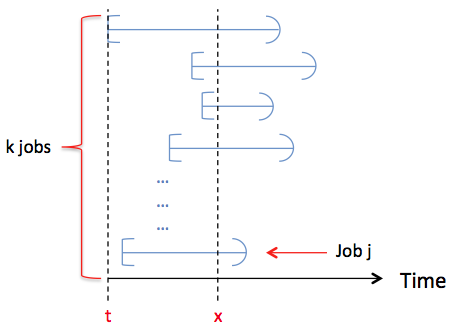
\includegraphics[width=0.4\textwidth]{../figures/claim1.png}
\caption{Our best option is to pick Job $j$}
\end{figure}

\begin{proof}
By assumption, from time $t$ to $x$, the choice of job within the $k$ jobs will not affect any other jobs outside of themselves. So, picking $j$ over $j'$ will not result in additional overlaps beyond the $k$ jobs. Now, suppose we construct an optimal solution by picking $j'$ instead of $j$. Then, we can obtain a feasible solution by replacing $j'$ by $j$. Hence, the optimal solution involving $j$ is at least as good as the solution generated by picking $j'$ out of the $k$ jobs.
\end{proof}

Let $\texttt{Chosen} = \{x_1, x_2, ..., x_m\}$ and $e_i = $ end time of job $x_i, \forall i \in \{1, 2, ..., m\}$. Then we can repeatedly apply the claim's argument at times $t = \{0, e_1, e_2, ... , e_{m-1}\}$ to show that the greedy algorithm is optimal.

\subsubsection{Algorithmic analysis}
Let $n$ be the number of jobs.\\
Then, the greedy algorithm takes $O(n \log_2 n + n^2) = O(n^2)$.\\
$O(n \log_2 n)$ comes from the sorting while $O(n^2)$ is due to $O(n)$ pairwise job comparisons to check for overlaps, each taking $O(n)$ time.

\subsection{Attempt to adapt to airport scheduling}
Motivated by what we learnt in interval scheduling, we came up with a na\"{\i}ve solution to airport gate scheduling. We attempted to modify the greedy interval scheduling algorithm as follows:

\begin{algorithm}[h!]
\begin{algorithmic}[1]
\caption{\textsc{GreedyAirportScheduling}(Flights)}
\label{alg:Greedy Airport Scheduling}
\STATE $Gates \leftarrow \emptyset$
\WHILE{$Flights$ not empty}
	\STATE $New\_Gate \leftarrow \textsc{GreedyIntervalScheduling(Flights)}$
	\STATE $Flights \leftarrow Flights \setminus New\_Gate$
	\STATE $Gates \leftarrow Gates \cup New\_Gate$
\ENDWHILE
\RETURN $Gates$
\end{algorithmic}
\end{algorithm}

\newpage
\subsubsection{Counter example}
Unfortunately, not surprisingly, greedy algorithms do not always produce optimal solutions. During our analysis of our na\"{\i}ve attempt, we found the following counter example, as shown in Figure \ref{fig:Counter-example}:

\begin{figure}[h!]
\centering
\begin{subfigure}[b]{\textwidth}
	\centering
	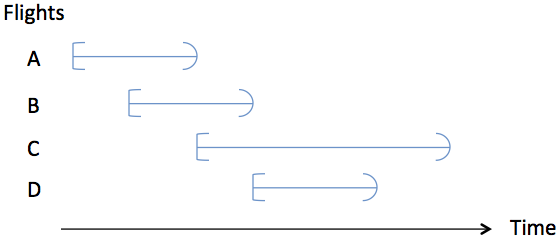
\includegraphics[width=0.4\textwidth]{../figures/counter-example.png}
	\caption{Counter example}
\end{subfigure}
	\centering
	\begin{subfigure}[b]{0.5\textwidth}
	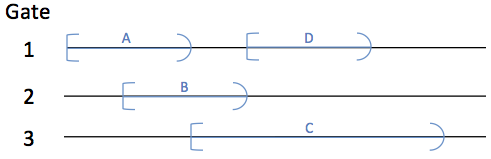
\includegraphics[width=\textwidth]{../figures/counter-example_naive.png}
	\caption{The na\"{\i}ve attempt uses 3 gates.}
\end{subfigure}~
	\centering
	\begin{subfigure}[b]{0.5\textwidth}
	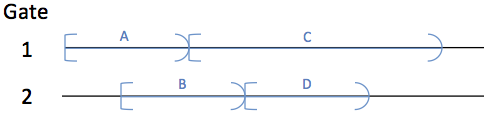
\includegraphics[width=\textwidth]{../figures/counter-example_opt.png}
	\caption{The optimal gate usage is 2.}
\end{subfigure}
\caption{Counter example to optimality of na\"{\i}ve attempt}
\label{fig:Counter-example}
\end{figure}

\section{Scheduling as a Graph Colouring problem}
Brushing aside our small setback, we took another look at the problem and realised that we can model our airport scheduling problem as a graph colouring problem. Let $G = (V,E)$ be the graph, where $V$ is the set of flights, and $(u,v) \in E$ means flights $u$ and $v$ have a collision in their schedules. In this formulation, finding a minimum colouring on the resultant graph $G$ will provide us an optimal solution to our original airport scheduling problem.

\begin{figure}[h!]
\centering
\begin{subfigure}[b]{0.4\textwidth}
	\centering
	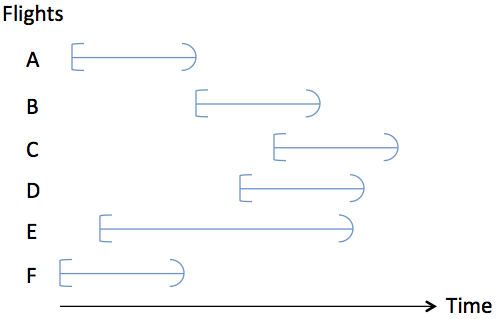
\includegraphics[width=\textwidth]{../figures/vanilla.png}
	\caption{Airport gate scheduling problem}
\end{subfigure}~
\begin{subfigure}[b]{0.4\textwidth}
	\centering
	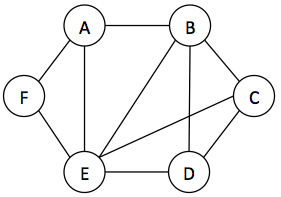
\includegraphics[width=\textwidth]{../figures/graph.png}
	\caption{Graph representation}
\end{subfigure}
\caption{Modelling airport gate scheduling as a graph}
\end{figure}

The problem of graph colouring is well explored in the Graph Theory branch of mathematics. In graph theory notation, \textbf{max degree vertex} $\Delta(G) = \max_{v \in V} deg(v)$ represents the highest degree of any vertex in the graph $G$, and \textbf{chromatic number} $\omega(G)$ means the minimum number of colours needed to colour the graph $G$. Clearly, $\omega(G) \leq \Delta(G) + 1$. Algorithm \ref{alg:Greedy Graph Colouring} presents a simple method to colour the graph in at most $\Delta(G) + 1$ colours.

\begin{algorithm}[h!]
\begin{algorithmic}[1]
\caption{\textsc{GreedyColour}(V, E)}
\label{alg:Greedy Graph Colouring}
\STATE $C \leftarrow$ Array of 0's of size $\vert V \vert$
\FOR{$v \leftarrow V$}
	\STATE $N \leftarrow \textsc{GetNeighbours(v, E)}$
	\STATE $c \leftarrow 1$
	\FOR{$n \leftarrow N$}
		\STATE $c \leftarrow \min(\{1, ... , \vert N \vert + 1\} \setminus \{c[n] : n \in N\})$
	\ENDFOR
	\STATE $C[v] \leftarrow c$
\ENDFOR
\RETURN $C$
\end{algorithmic}
\end{algorithm}

\subsection{Proof of correctness}
Observe that we always try to assign the smallest `free'/unused colour (from 1 to $\vert N \vert$ + 1). We claim that throughout the entire algorithm, the following invariant holds.

\hspace{0pt}
\begin{claim}
For any vertex v, $C[v] = c \leq deg(v) + 1$.
\end{claim}
\begin{proof}
In the worst case, all neighbours of $v$ use different colours, from 1 up to $deg(v)$. So, $v$ has to use the colour $deg(v) + 1$.
\end{proof}

Since this holds for all vertices, it holds for the vertex with degree $\Delta(G)$. Hence, the algorithm gives us a colouring with at most $\Delta(G) + 1$ colours.

\subsection{Proof of optimality}
Here, we claim that after transforming our problem into a graph, Algorithm \ref{alg:Greedy Graph Colouring} provides us with an optimal schedule.

Observe that in interval scheduling, if there are $k$ overlaps at any time $t$, then we can at most include one of the $k$ flights. In a graph, these overlaps would be represented by a $k$-clique. It is easy to see that $\Delta(G) + 1$ will simply be the maximum number of overlaps. Since we need at least $\Delta(G) + 1$ colours to resolve this maximum overlap, and our algorithm provides such a colouring, it is optimal.

\subsection{Algorithmic analysis}
The greedy algorithm takes $O(|V| + |E|)$.
This is because we considered each vertex and edge once in the rest of the entire algorithm\footnote{We can efficiently check the neighbours of a vertex if we store the graph in an adjacency list.}.

\section{Interval partitioning}
Despite having an optimal solution, it can be time/space consuming to store the data in a graph before we can actually execute the above algorithm. So, we looked for alternative solutions.

In our search, we came across a problem known as ``Resource Allocation'' or ``Interval Partitioning'' which describes exactly the airport gate scheduling problem\footnote{References:\\
\url{http://www.cs.rit.edu/~zjb/courses/800/lec8.pdf}\\
\url{http://courses.cs.vt.edu/cs5114/spring2009/lectures/lecture04-greedy-scheduling.pdf}}, but in a different context.

The problem can be formulated as follows: Given a set of $n$ jobs with their start and finish times, find a partition of size $k$ such that each set of jobs in the partitions do not overlap and $k$ is minimized. In our case, ``jobs'' refer to flights and ``partitions'' refer to ``gates''.

Algorithm \ref{alg:Greedy Interval Partitioning} is the greedy, yet optimal, algorithm for the interval partitioning problem, which minimizes $\vert \texttt{Partition} \vert$ while satisfying the condition that all jobs in the partitions do not overlap. We pass in an empty list as \texttt{Partition}. The reason for using it as a parameter is to allow us to pass in non-empty lists as initial partitions\footnote{This allows us to schedule with extra gates during the experiments in Section \ref{sec:Experiments}.}.

\begin{algorithm}[h!]
\begin{algorithmic}[1]
\caption{\textsc{GreedyIntervalPartitioning}(Jobs, Partiton)}
\label{alg:Greedy Interval Partitioning}
\STATE $J \leftarrow \textsc{SortByEarliestStartTime(Jobs)}$
\STATE $count \leftarrow 0$
\FOR{$j \in J$}
	\IF{$j$ does not overlap with all existing jobs in some Partition $k$}
	\label{line:Correctness}
		\STATE $\texttt{Partition}[k] \leftarrow \texttt{Partition}[k] \cup \{j\}$
	\ELSE
		\STATE $count \leftarrow count + 1$
		\STATE $\texttt{Partition}.append(\emptyset)$
		\STATE $\texttt{Partition}[count] \leftarrow \texttt{Partition}[count] \cup \{j\}$
	\ENDIF
\ENDFOR
\RETURN \texttt{Partition}
\end{algorithmic}
\end{algorithm}

For our purposes, when given a choice of possible partitions in Line \ref{line:Correctness}, we choose the one with the most slack. This allows us to extend our algorithm to the case when we are given extra gates to begin with.

\subsection{Proof of correctness}
By construction, the check in Line \ref{line:Correctness} of the algorithm will ensure that the resultant partitions do not have overlapping jobs.

\subsection{Proof of optimality}
Let $d$ be the maximum number of overlaps at any point in time. i.e. $d = \Delta(G) - 1$. Since we know that $\vert \texttt{Partition} \vert \geq d$, if we can show that $\vert \texttt{Partition} \vert = d$, then the algorithm is optimal.

\hspace{0pt}
\begin{claim}
$\vert \texttt{Partition} \vert = d$
\end{claim}
\begin{proof}\hspace{0pt}\\
Recall that $\vert \texttt{Partition} \vert \geq d$ and $\vert \texttt{Partition} \vert = count$ within the algorithm.\\
Suppose not. Then let us assume that $\vert \texttt{Partition} \vert > d$.\\
Then at some point in our algorithm, $d = count$. Consider the job $j$ that caused us to increment $count$ (i.e. We create a $(count + 1)^{th}$ partition for $j$).\\
By the algorithm, we only do so when all the current partitions $\texttt{Partition}[1]$ up to $\texttt{Partition}[count]$ all have overlaps with job $j$. This implies that at the start time of job $j$, we have $(count + 1) \geq d + 1 > d$ number of overlaps.\\
But this contradicts that $d$ is the maximum number of overlaps at any point in time!\\
So, $\vert \texttt{Partition} \vert > d$ is impossible. Hence, we have that $\vert \texttt{Partition} \vert = d$.
\end{proof}

\subsection{Algorithmic analysis}
Let $n$ be the number of jobs and $d$ be the maximum number of overlaps at any point in time. Then, the algorithm takes $O(n \log_2 n + n \cdot d) = O(n \cdot (\log_2 n + d))$ time to run.\\
This is because we take $O(n \log_2 n)$ time to sort the jobs. Then, for every job, we compare with each existing partition, which takes $O(d)$ time each.

\section{Interesting observations}
The most interesting observation is probably that the number of gates required is exactly $d$, where $d$ is the maximum number of overlaps at any point in time. As we discussed before, it is an obvious lower bound since we need at least one gate per plane when we incur $d$ overlaps. However, we were initially pleasantly surprised that this lower bound was actually attainable.

On hindsight, if we formulated the problem in to graph colouring problem, then the result would not have been so surprising after all. Graph colouring gives us an obvious upper bound of $\Delta(G) + 1$ that actually equals $d$. It was nice to see different fields of study come together.

\chapter{Airport Gate Scheduling with Delays}

In real world situations, delays are usually inevitable. In our context, a delay happens when the actual flight arrival or departure time differs from the scheduled one. It can be a positive or negative amount of delay (Negative delay indicates earlier arrival/departure than expected). In this chapter, we consider the same problem of airport gate scheduling and explore how delay affects our scheduling.

\begin{figure}[h!]
\centering
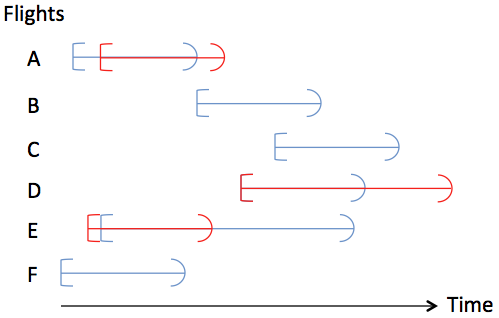
\includegraphics[width=0.4\textwidth]{../figures/delays.png}
\caption{Illustration of delays:\\ Flights A and D have positive delay while Flight E has negative delay.}
\end{figure}

\section{Definitions}
Before we begin, let us first lay out some definitions.

\subsection{Delays, Gate Collision and Re-assignments}
\subsubsection{Delay (Measured in minutes)}
A delay is an integer $d \in \mathbb{Z}$, which can be either positive or negative. It is the time difference between the scheduled flight arrival/departure and the actual one.

We usually have to plan based on the scheduled timings and then make impromptu changes to the schedule as delays occur. A plane that has non-zero delay is also called a delayed plane.

\subsubsection{Gate Collision}
A gate collision happens when using the original schedule and the delayed planes, two planes are assigned to the same gate at the same time.

\subsubsection{Re-assignment}
A re-assignment occurs when we move a Plane $p$ from some Gate $i$ to some Gate $j$. We need to do this when a gate collision happens when we take into account the delay of Plane $p$.

\subsubsection{Relation between gate collisions and re-assignments}
While it is clear that gate collisions are bound to cause re-assignments, it is perhaps less obvious that re-assignments can also cause gate collisions. Consider the following scenario where we put into effect Plane $i$'s delay, which caused a collision with Plane $j$:

\begin{figure}[h!]
\centering
\begin{subfigure}[b]{0.5\textwidth}
	\centering
	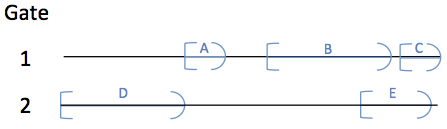
\includegraphics[width=\textwidth]{../figures/options_original.png}
	\caption{Original schedule}
\end{subfigure}~
\begin{subfigure}[b]{0.5\textwidth}
	\centering
	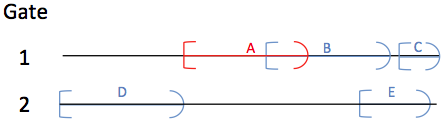
\includegraphics[width=\textwidth]{../figures/options_delay.png}
	\caption{Flight A is delayed}
\end{subfigure}

\begin{subfigure}[b]{0.3\textwidth}
	\centering
	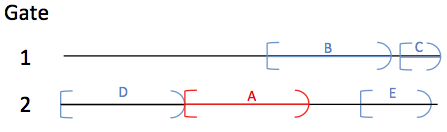
\includegraphics[width=\textwidth]{../figures/options1.png}
	\caption{Shift Plane A}
\end{subfigure}~
\begin{subfigure}[b]{0.3\textwidth}
	\centering
	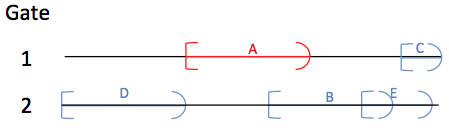
\includegraphics[width=\textwidth]{../figures/options2.png}
	\caption{Shift Plane B}
\end{subfigure}~
\begin{subfigure}[b]{0.3\textwidth}
	\centering
	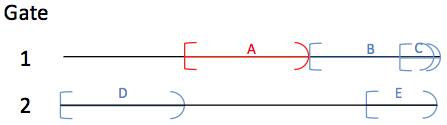
\includegraphics[width=\textwidth]{../figures/options3.png}
	\caption{Delay Plane B}
\end{subfigure}
\caption{Illustration of the various options of resolving gate collisions}
\end{figure}

Assuming we have sufficient resources, one method that always works is to just open a new gate and assign either Plane $i$ or Plane $j$ there. That will definitely solve the issue. However, resource is usually tight, so we consider the the following options:
\begin{enumerate}[(a)]
\item Shift Plane $i$ to another existing gate
\item Shift Plane $j$ to another existing gate
\item Keep both planes in the same gate. Push Plane $j$'s usage of the gate backwards (push back the take-off time or ask it to circle around in the air for a bit before landing)
\end{enumerate}
Each of these options are recursive in nature, where we keep picking an option until we finally manage to get rid of all gate collisions due to Plane $i$'s delay.

There is no simple method to determine before hand which of the above options is optimal since future planes can be delayed as well. In the worst case scenario, while resolving the single gate collision due to Plane $i$'s delay, we could potentially cause a whole lot more gate collisions between other planes. Unfortunately, it is non-trivial to predict beforehand which of the options is the best.

\label{Subsection: Slack}
\subsection{Slack}
The key concern when scheduling with delays is to minimise the number of gate collisions and re-assignments. Unfortunately, unless we have an oracle, we cannot measure or predict beforehand. The next best thing we can do is to employ an auxiliary/intermediary variable and optimize over that.

Slack is a useful notion that serves this purpose. Intuitively, a schedule with more slack would be more robust to perturbation in the flight schedules since the slack will likely `absorb' delays and avoid gate collisions.

For illustration purposes, let us consider the extreme cases in Figure \ref{fig:Extreme}. When all planes and gates are packed like sardines in a can, a slight amount of delay in any of the planes would cause a re-scheduling catastrophe. On the other hand, if we assign a gate to every single plane, then we are guaranteed that no amount of delay will cause any form of gate collisions.

\begin{figure}[h!]
\centering
\begin{subfigure}[b]{0.5\textwidth}
	\centering
	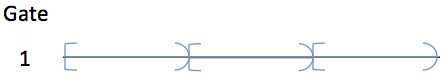
\includegraphics[width=\textwidth]{../figures/extreme0.png}
	\caption{0 slack: No free space between planes}
\end{subfigure}~
\begin{subfigure}[b]{0.5\textwidth}
	\centering
	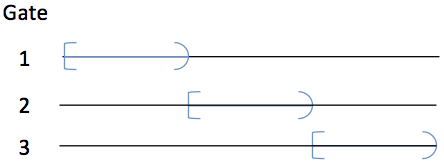
\includegraphics[width=\textwidth]{../figures/extreme_max.png}
	\caption{Maximum slack: 1 gate per plane}
\end{subfigure}
\caption{Illustration of the extreme slack cases}
\label{fig:Extreme}
\end{figure}

While it is easy to convince ourselves that slack could be useful for our purposes, there are 2 more tasks at hand: (a) Proving that maximizing slack guarantees minimising gate collisions/re-assignment; and (b) Giving a working definition of slack.

For (a), we are unable to formalize the problem hence we did not manage to tackle it. We are also unable to find any work that seem to have made progress on this. So, for now, let us just trust that our intuition that ``greater slack implies lower number of gate collisions'' is reasonable.

As for (b), we employ a rather strict working definition of slack, and we aim to maximize it: Slack is the minimum free time between any pair of flights across all gates. We show a graphical example in Figure \ref{fig:Slack definition}.

\begin{figure}[h!]
\centering
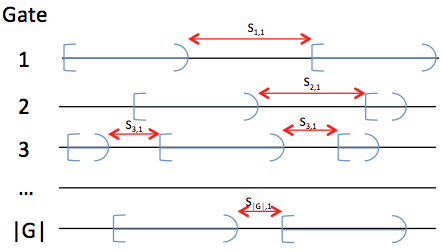
\includegraphics[width=0.7\textwidth]{../figures/slack.png}
\caption{Slack = $\min x_{i,j}, \forall i,j$}
\label{fig:Slack definition}
\end{figure}

Although in this project we aim to maximise slack, it is perhaps important to point out that reality is much more complicated. Companies often want to minimize slack in order to reduce wastage of resources such as idle gate time. At the same time, they wish to minimize gate collisions. This leads to an interesting trade-off that we will not explore in this project.

\newpage
\section{Our method}
\subsection{Handling gate re-assignments}
We first calculate the optimal schedule based on ``scheduled arrival/departures''. Then, we consider the following scenarios:
\begin{enumerate}
\item With random probability $p$, add random delay in the range $[\texttt{minD}, \texttt{maxD}]$ to each plane
\item Use the ``actual arrival/departures'' from the data
\end{enumerate}
Algorithm \ref{alg:Rescheduling} describes our approach for rescheduling. We will explore the above two situations in Section \ref{sec:Experiments}.

\begin{algorithm}[h!]
\begin{algorithmic}[1]
\caption{\textsc{Rescheduling}(Schedule, Planes)}
\label{alg:Rescheduling}
\STATE $P \leftarrow \textsc{SortByEarliestDelayedStartTime(Planes)}$
\STATE $\texttt{Overflow} \leftarrow []$
\FOR{$p \in P$}
	\IF{$p$ collides in current schedule}
		\STATE $\text{Free Gate with most slack} \leftarrow \texttt{Schedule} \cup \texttt{Overflow}$
		\IF{No such free gates}
			\STATE Assign $p$ to a new gate
			\STATE Assign newly created gate to \texttt{Overflow}
		\ELSE
			\STATE Reassign $p$ to free gate
		\ENDIF
	\ENDIF
\ENDFOR
\RETURN $\texttt{Schedule} \cup \texttt{Overflow}$
\end{algorithmic}
\end{algorithm}

\subsection{Scheduling with extra gates before hand}
Suppose we are now given $G$ gates to begin our assignment. We simply pass in a list of $G$ empty gates instead of an empty list to the parameter \texttt{Partition} in our Algorithm \ref{alg:Greedy Interval Partitioning}.

\chapter{Implementation and experiments}
\section{Dataset}
We obtain our dataset from the ``Research and Innovative Technology Administration Bureau of Transportation Statistics'' (RITA)\footnote{Database download:\\ \url{http://www.transtats.bts.gov/DL_SelectFields.asp?Table_ID=236}.\\ Attribute description:\\ \url{http://www.transtats.bts.gov/TableInfo.asp?Table_ID=236}}. The database provides us with 471950 flight details for the month of January 2014. Table \ref{tab: RITA} explains the attributes which we extracted from the database.

Some flight entries have missing fields so we omit those in our computation. We also filter away airports that are not busy ($<100$ flights) since they usually produce anomalous results in our experiments. As a result, we only look at a total of 736601 flights\footnote{Flights are double counted: once for departure and once for arrival.} and 1788 airports across the entire month of January 2014\footnote{Without filtering airports to have at least 100 flights, we would have been considering a total of 880906 flights and 9111 airports. But we feel that the filtered dataset is still reasonably large enough.}.


\label{tab: RITA}
\begin{table}[h!]
\center
\begin{tabular}{|c|c|}
\hline
Header in dataset & Attribute\\
\hline
\texttt{FL\_DATE} & Date of flight\\
\texttt{ORIGIN\_AIRPORT\_ID} & Identifier of airport which flight took off from\\
\texttt{DEST\_AIRPORT\_ID} & Identifier of airport which flight landed in\\
\texttt{CRS\_DEP\_TIME} & Scheduled departure time\\
\texttt{DEP\_TIME} & Actual departure time\\
\texttt{DEP\_DELAY} & (Actual - Scheduled) departure time\footnotemark{}\\
\texttt{CRS\_ARR\_TIME} & Scheduled arrival time\\
\texttt{ARR\_TIME} & Actual arrival time\\
\texttt{ARR\_DELAY} & (Actual - Scheduled) arrival time\footnotemark{}\\
\hline
\end{tabular}
\caption{Flight Attributes}
\end{table}
\footnotetext[4]{Negative delay means earlier departure.}
\footnotetext[5]{Negative delay means earlier arrival.}

We actually do not make use of the attributes \texttt{DEP\_DELAY} and \texttt{ARR\_DELAY}. We just pulled them out of the database for referencing purposes.

\section{Implementation of algorithms}
We provide the source code of our implementation and experiments in the Github repository here\footnote{\url{https://github.com/sozos/RAS}}. In the repository, besides our report, you will find the following source programs:

\begin{table}[h!]
\center
\begin{tabular}{|c|c|}
\hline
Name & Purpose\\
\hline
data.py & Processes data from RITA\\
experiments.py & Script that runs our experiments\\
schedule.py & Assigns and re-assigns flights to gates\\
util.py & Helper functions (e.g. time manipulation)\\
Gate.py & Gate class\\
FlightInfo.py & Flight info class\\
Interval.py & Interval class\\
test\_data.csv & Data pulled from RITA\\
\hline
\end{tabular}
\caption{Project Files}
\end{table}

In our entire project, we treat time in terms of minutes within a day. That is to say, time will be represented by a natural number from 0 to 1439.

\section{Experiments}
\label{sec:Experiments}
From empirical data, we observe that the probability of an actual delay\footnote{The fraction of flights that have differing scheduled and actual departure/arrival times} $p$ is approximately 0.948 (rounded to 3 decimal places). So, if we want to introduce random delays to the data, we would delay each plane with a random delay\footnote{In minutes} in the range \texttt{[minDelay, maxDelay]}\footnote{\texttt{minDelay} can be negative} with probability $p$. In our experiments, we use a symmetric range for random delay. That is to say, we set \texttt{|minDelay| = |maxDelay|}.

\subsection{Scenario 1 - Establishing a basic relationship}
In this scenario, we investigate the relationship between the number of flights and the number of gates needed.

While our optimal algorithm (Algorithm \ref{alg:Greedy Interval Partitioning}) tells us that the number of gates is exactly the highest number of overlaps in any point in time, we cannot use that to answer this query since we do not know the distribution of overlaps in flights.

Therefore, we compute the number of flights and gates needed for all the airports, across all days, within the month of January.

\begin{figure}[h!]
\centering
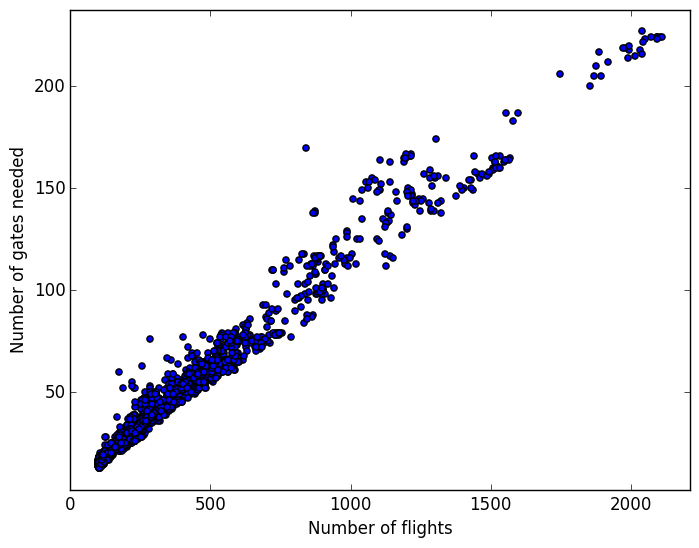
\includegraphics[width=0.8\textwidth]{../graph/2b.png}
\caption{Relationship between number of flights and number of gates needed}
\end{figure}

Our findings show that there is a somewhat linear relationship, which makes intuitive sense.

% ``2b''
% ``How many gates are needed?''
% ``Is there any relationship between the number of flights and the number of gates needed?''
% Are the number of flights somehow correlated to the number of gates required?
% For loop on dates + Plot graph

\newpage
\subsection{Scenario 2 - Artificial random delays}
In this scenario, given an optimal schedule using the scheduled times of flights, we wonder how much random delay is needed before we observe a collision.

To do so, we introduce random delay to perturb the flight timings. Clearly, the amount of delay that can be tolerated would depend somewhat on how packed the schedule is. Hence, we compare this value against our definition of slack (as per Subsection \ref{Subsection: Slack}) across all airports, across all days, within the month of January.

\begin{figure}[h!]
\centering
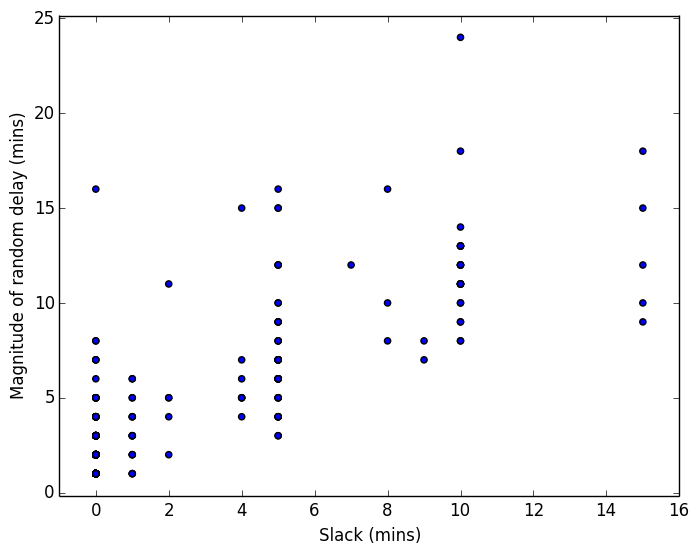
\includegraphics[width=0.8\textwidth]{../graph/3ai.png}
\caption{Smallest magnitude of random delay before first collision, with respect to slack at airport}
\label{fig:SmallestDelay}
\end{figure}

Notice that the bottom right section of Figure \ref{fig:SmallestDelay} is devoid of data points. That tells us empirically that as minimum slack increases, we have some sort of guarantee on the minimum magnitude of random delay that is needed before we see any collisions.

% ``3a(i)''
% ``How much random delay is needed before we see a collision?''
% Perturb data with artificial delay
% Amount of delays before collisions happen (for which day?)

Now, we explore a scenario similar to the previous, but from a slightly different point of view. Instead of increasing the magnitude of random delay until we observe a collision, we consider the number of gate collisions given a fixed level of random delay.

From the dataset, we observe that the mean magnitude of delay is 23.68091 minutes (rounded to 5 decimal places), so we introduce random delays in the range \texttt{[-24, 24]} across all airports, across all days, within the month of January.

\begin{figure}[h!]
\centering
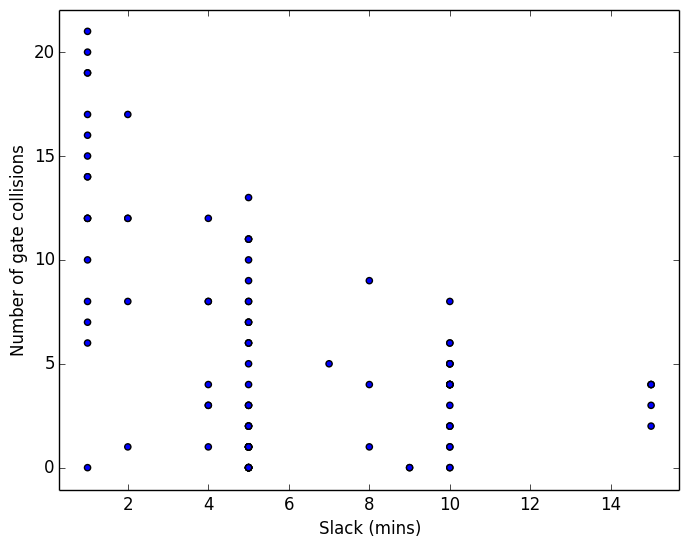
\includegraphics[width=0.8\textwidth]{../graph/3aii.png}
\caption{Number of gate collisions when random delay is introduced, with respect to slack at airport}
\label{fig:3aii}
\end{figure}

\newpage
Obviously when we have no slack, the number of collisions are astronomical. There are 1683 such cases with the maximum number of gate collisions being 702. Thankfully, we see that the number of collisions drops drastically when we have just 1 minute of slack, as shown in Figure \ref{fig:3aii}. We can vaguely see the outline of a reciprocal shape in the figure as well.

% ``3a(ii)''
% ``For a given level of random delay, how many gate collisions do we see?''
% Perturb data with artificial delay
% With a fixed amount of delay, how much collisions will happen?

\newpage
\subsection{Scenario 3 - Investigating actual delays}
Having played with artificial delays, we now turn our attention to the actual delays from the real dataset. We first look at the number of gate collisions that occur in reality.

\begin{figure}[h!]
\centering
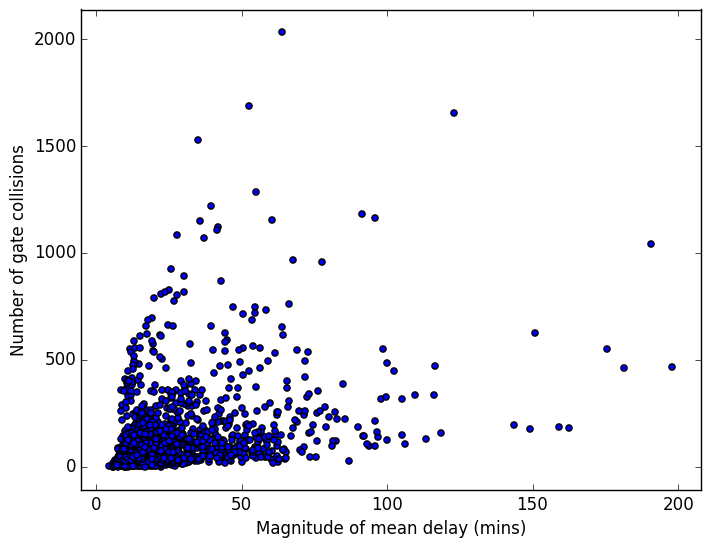
\includegraphics[width=0.8\textwidth]{../graph/3aiii.png}
\caption{Number of collisions w.r.t. the magnitude of mean delay at the airport \protect\footnotemark}
\label{fig:3aiii}
\end{figure}
\footnotetext{Magnitude of mean delay of an airport = $\frac{\sum|\texttt{actual flight time} - \texttt{scheduled flight time}|}{\texttt{Number of flights at airport}}$}

Observe that there is no clear trend in Figure \ref{fig:3aiii} except that most airports cluster in the bottom left portion of the graph. Perhaps mean delay is not indicative of the number of gate collisions that can happen at an airport. We looked at the raw data and there are certain cases where planes are delayed for hours. Situations like those could result in tons of gate collisions, especially if the airport is packed with low amount of slack.

Next, we run our rescheduling algorithm and compare it against the ideal case (where an oracle provides us the actual departure/arrival time and we just run our optimal scheduling algorithm on that). Below, we show our results with relation to the mean amount of delay for each airport, across all days, within the month of January.

\begin{figure}[h!]
\centering
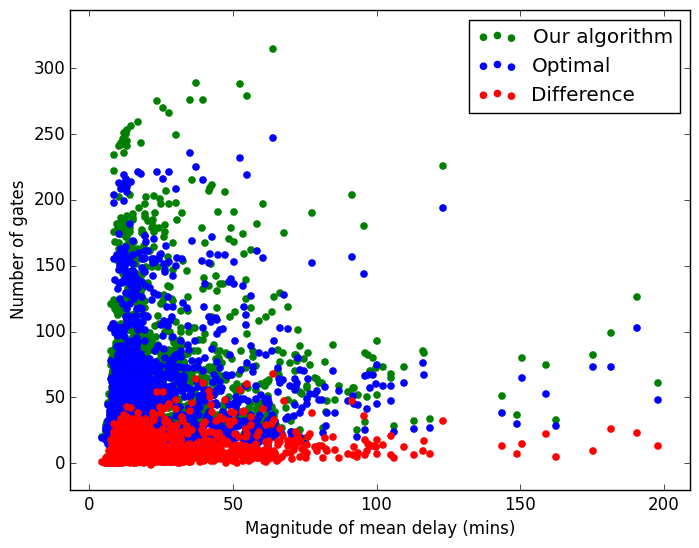
\includegraphics[width=0.8\textwidth]{../graph/3bi.png}
\caption{Number of gates w.r.t. the magnitude of mean delay at the airport}
\label{fig:3bi}
\end{figure}

\begin{figure}[h!]
\centering
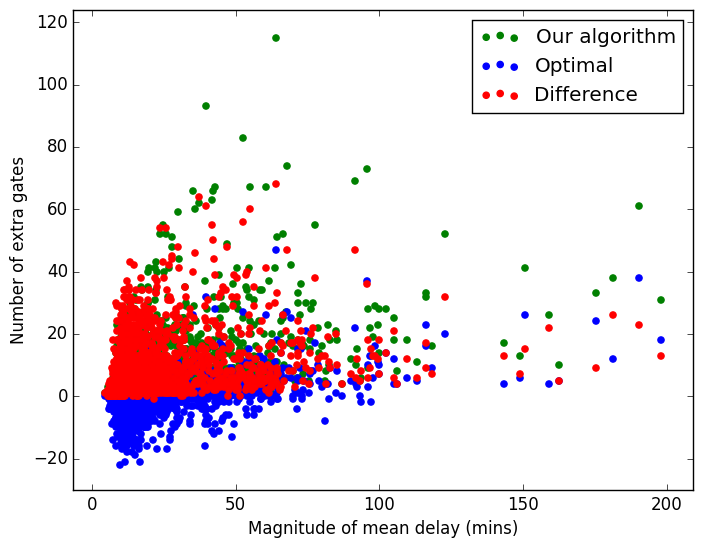
\includegraphics[width=0.8\textwidth]{../graph/3bii.png}
\caption{Number of extra gates w.r.t. the magnitude of mean delay at the airport}
\label{fig:3bii}
\end{figure}

For Figures \ref{fig:3bi} and \ref{fig:3bii}, we overlay 3 different sets of data for visualization purposes. On each graph, we show: (i) Result from our rescheduling algorithm; (ii) Result from the oracle scheduling; (iii) The difference between our result and the oracle's. As we can see, our rescheduling algorithm fares pretty well.

Note that for many situations with low magnitude of mean delay, the optimal algorithm actually took less gates than the optimal gates required in the original schedule (hence ``negative extra gates''). In those situations, a ``difference'' comparison is pretty meaningless.

% ``3a(iii)''
% ``Now, use the actual delays from the real dataset. How many gate collisions do we see?''

% ``3b(i)''
% ``For the delays in the dataset, how many gates do we need?''

% ``3b(ii)''
% ``How does the number of extra gates needed scale with the delays?''

% Evaluate performance of our re-scheduling
% With actual data, how many more gates do we need?
% Compare with optimal number of gates, assuming we knew the delays before hand

\subsection{Scenario 4 - Minimizing number of gate re-assignments}
Lastly, we consider the situation where we are given $E$ extra gates on top of the minimum number of gates required to plan the scheduled timings.

As a basis for comparision, we consider the range of extra gates from none, to having an extra gate per plane\footnote{Recall that when we have 1 gate per plane, then we will not have any collisions.}. We denote this as the ``percentage of extra gates''. Note that the number of extra gates given at the start is not a fixed constant but will vary based on the number of flights at the airport.

Figures \ref{fig:4i} and \ref{fig:4ii} compare the number of reassignments and percentage of success across all airports in our dataset\footnote{We consider a success for an airport when we are able to reschedule all flights without employing any overflow gates.} against the percentage of extra gates.

\begin{figure}[h!]
\centering
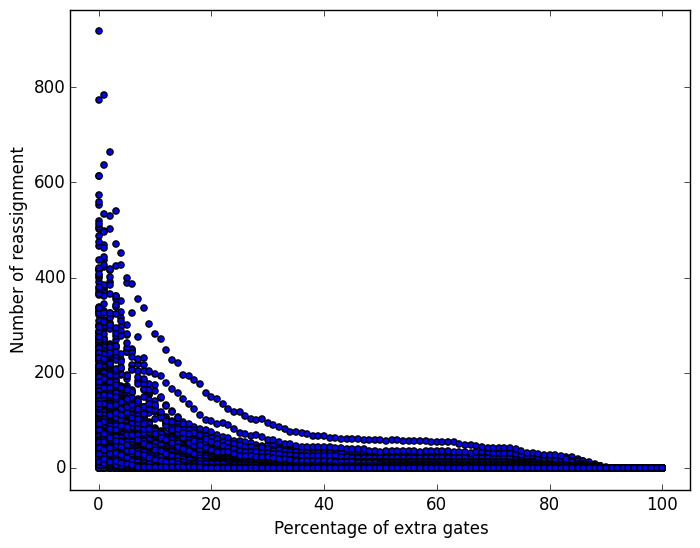
\includegraphics[width=0.8\textwidth]{../graph/4i.png}
\caption{Number of gate assignments w.r.t. Percentage of extra gates}
\label{fig:4i}
\end{figure}

\begin{figure}[h!]
\centering
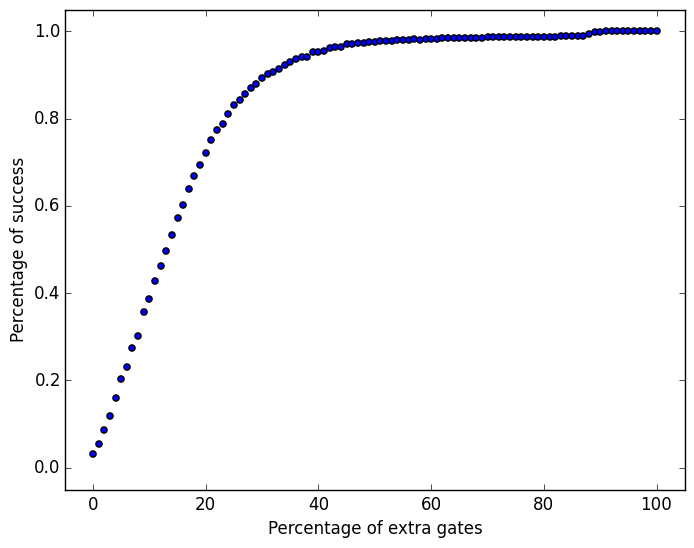
\includegraphics[width=0.8\textwidth]{../graph/4ii.png}
\caption{Number of extra gate assignments w.r.t. Percentage of extra gates}
\label{fig:4ii}
\end{figure}

\newpage
As expected, Figures \ref{fig:4i} and \ref{fig:4ii} display a reciprocal shape and logarithmic shape respectively. From Figure \ref{fig:4ii}, we can state with relative confidence that ``using extra gates with at least 40\% of the total number of flights, we can attain 95\% success rate in dealing with delays''.

% ``4(i)''
% ``Show, via experiment, that this minimizes the number of gate reassignments''
% With actual data, start with E extra gates, how many collisions do we see?

% ``4(ii)''
% ``Prove that your assignment can handle a certain level of delay''

\chapter{Conclusion}
In this project, we investigated the problem of robust airport scheduling.

To solve the vanilla airport scheduling problem, we first looked at the literature of interval scheduling and graph colouring before we settled on using the optimal interval partitioning algorithm. In this portion, we learn that by formulating the problem into different fields, we can obtain both obvious upper and lower bounds for our problem.

While we optimally solve the vanilla airport scheduling problem, things get hairy when we consider a more realistic situation where flights get delayed. For this problem, we first came up with ways to reschedule flights that cause collisions with a given original schedule. To aid us, we investigated ``slack'' as an auxiliary measurable variable in place of the vague notion of ``delay''.

Lastly, we conducted computational experiments based on our findings and explored a few interesting scenarios using data from RITA.

\end{document}
